% Created by tikzDevice version 0.10.1.2 on 2018-04-07 16:32:09
% !TEX encoding = UTF-8 Unicode
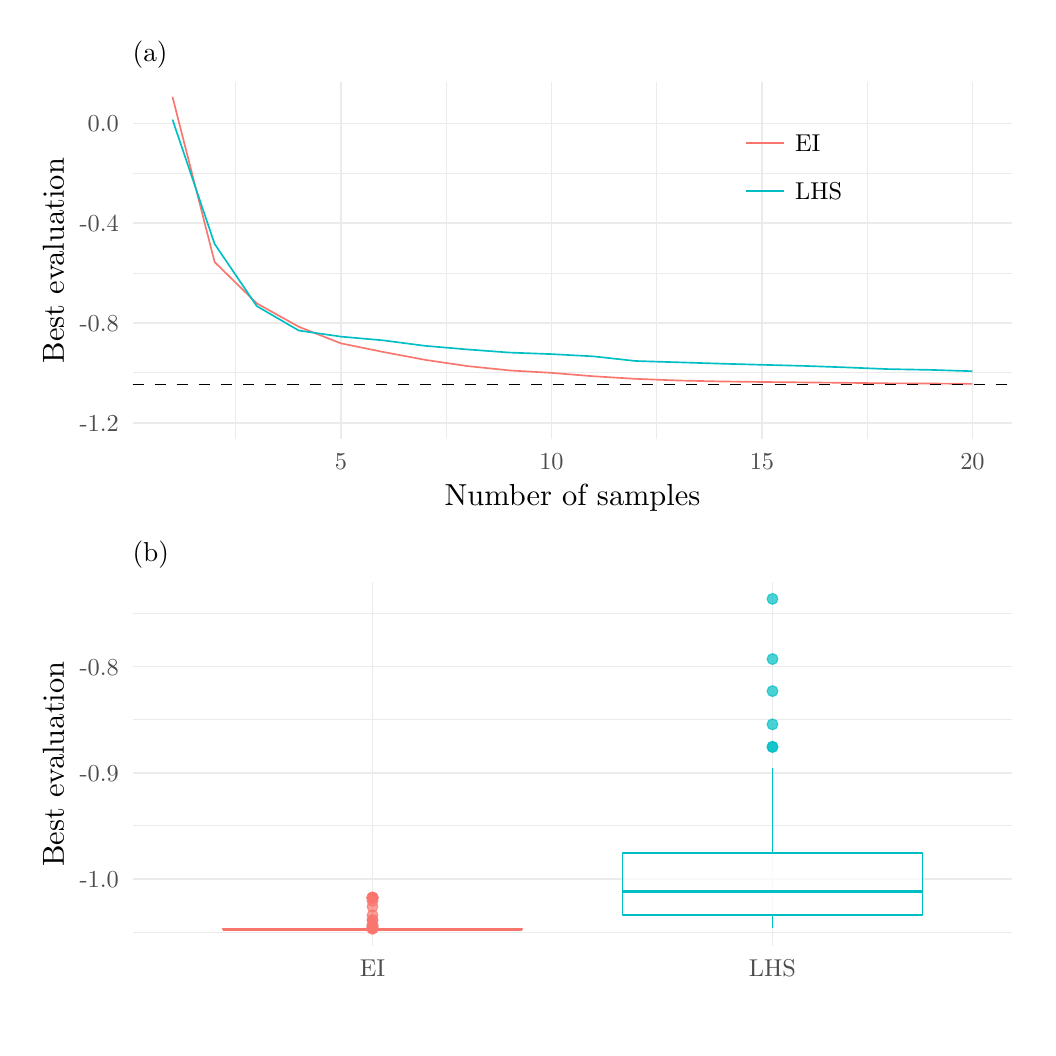
\begin{tikzpicture}[x=1pt,y=1pt]
\definecolor{fillColor}{RGB}{255,255,255}
\path[use as bounding box,fill=fillColor,fill opacity=0.00] (0,0) rectangle (361.35,361.35);
\begin{scope}
\path[clip] ( 37.88,212.76) rectangle (355.85,341.59);
\definecolor{drawColor}{gray}{0.92}

\path[draw=drawColor,line width= 0.3pt,line join=round] ( 37.88,236.63) --
	(355.85,236.63);

\path[draw=drawColor,line width= 0.3pt,line join=round] ( 37.88,272.67) --
	(355.85,272.67);

\path[draw=drawColor,line width= 0.3pt,line join=round] ( 37.88,308.70) --
	(355.85,308.70);

\path[draw=drawColor,line width= 0.3pt,line join=round] ( 75.15,212.76) --
	( 75.15,341.59);

\path[draw=drawColor,line width= 0.3pt,line join=round] (151.22,212.76) --
	(151.22,341.59);

\path[draw=drawColor,line width= 0.3pt,line join=round] (227.29,212.76) --
	(227.29,341.59);

\path[draw=drawColor,line width= 0.3pt,line join=round] (303.36,212.76) --
	(303.36,341.59);

\path[draw=drawColor,line width= 0.6pt,line join=round] ( 37.88,218.61) --
	(355.85,218.61);

\path[draw=drawColor,line width= 0.6pt,line join=round] ( 37.88,254.65) --
	(355.85,254.65);

\path[draw=drawColor,line width= 0.6pt,line join=round] ( 37.88,290.69) --
	(355.85,290.69);

\path[draw=drawColor,line width= 0.6pt,line join=round] ( 37.88,326.72) --
	(355.85,326.72);

\path[draw=drawColor,line width= 0.6pt,line join=round] (113.19,212.76) --
	(113.19,341.59);

\path[draw=drawColor,line width= 0.6pt,line join=round] (189.26,212.76) --
	(189.26,341.59);

\path[draw=drawColor,line width= 0.6pt,line join=round] (265.33,212.76) --
	(265.33,341.59);

\path[draw=drawColor,line width= 0.6pt,line join=round] (341.40,212.76) --
	(341.40,341.59);
\definecolor{drawColor}{RGB}{248,118,109}

\path[draw=drawColor,line width= 0.6pt,line join=round] ( 52.33,336.34) --
	( 67.55,276.67) --
	( 82.76,261.74) --
	( 97.98,253.27) --
	(113.19,247.27) --
	(128.40,244.18) --
	(143.62,241.31) --
	(158.83,239.07) --
	(174.04,237.50) --
	(189.26,236.62) --
	(204.47,235.38) --
	(219.69,234.45) --
	(234.90,233.86) --
	(250.11,233.51) --
	(265.33,233.32) --
	(280.54,233.16) --
	(295.76,233.02) --
	(310.97,232.83) --
	(326.18,232.77) --
	(341.40,232.63);
\definecolor{drawColor}{RGB}{0,191,196}

\path[draw=drawColor,line width= 0.6pt,line join=round] ( 52.33,328.13) --
	( 67.55,283.20) --
	( 82.76,260.76) --
	( 97.98,251.90) --
	(113.19,249.71) --
	(128.40,248.36) --
	(143.62,246.38) --
	(158.83,245.08) --
	(174.04,243.95) --
	(189.26,243.39) --
	(204.47,242.57) --
	(219.69,240.90) --
	(234.90,240.43) --
	(250.11,239.95) --
	(265.33,239.53) --
	(280.54,239.13) --
	(295.76,238.59) --
	(310.97,237.97) --
	(326.18,237.69) --
	(341.40,237.21);
\definecolor{drawColor}{RGB}{0,0,0}

\path[draw=drawColor,line width= 0.6pt,dash pattern=on 4pt off 4pt ,line join=round] ( 37.88,232.40) -- (355.85,232.40);
\end{scope}
\begin{scope}
\path[clip] (  0.00,  0.00) rectangle (361.35,361.35);
\definecolor{drawColor}{gray}{0.30}

\node[text=drawColor,anchor=base east,inner sep=0pt, outer sep=0pt, scale=  0.88] at ( 32.93,215.58) {-1.2};

\node[text=drawColor,anchor=base east,inner sep=0pt, outer sep=0pt, scale=  0.88] at ( 32.93,251.62) {-0.8};

\node[text=drawColor,anchor=base east,inner sep=0pt, outer sep=0pt, scale=  0.88] at ( 32.93,287.66) {-0.4};

\node[text=drawColor,anchor=base east,inner sep=0pt, outer sep=0pt, scale=  0.88] at ( 32.93,323.69) {0.0};
\end{scope}
\begin{scope}
\path[clip] (  0.00,  0.00) rectangle (361.35,361.35);
\definecolor{drawColor}{gray}{0.30}

\node[text=drawColor,anchor=base,inner sep=0pt, outer sep=0pt, scale=  0.88] at (113.19,201.74) {5};

\node[text=drawColor,anchor=base,inner sep=0pt, outer sep=0pt, scale=  0.88] at (189.26,201.74) {10};

\node[text=drawColor,anchor=base,inner sep=0pt, outer sep=0pt, scale=  0.88] at (265.33,201.74) {15};

\node[text=drawColor,anchor=base,inner sep=0pt, outer sep=0pt, scale=  0.88] at (341.40,201.74) {20};
\end{scope}
\begin{scope}
\path[clip] (  0.00,  0.00) rectangle (361.35,361.35);
\definecolor{drawColor}{RGB}{0,0,0}

\node[text=drawColor,anchor=base,inner sep=0pt, outer sep=0pt, scale=  1.10] at (196.87,188.67) {Number of samples};
\end{scope}
\begin{scope}
\path[clip] (  0.00,  0.00) rectangle (361.35,361.35);
\definecolor{drawColor}{RGB}{0,0,0}

\node[text=drawColor,rotate= 90.00,anchor=base,inner sep=0pt, outer sep=0pt, scale=  1.10] at ( 13.08,277.17) {Best evaluation};
\end{scope}
\begin{scope}
\path[clip] (  0.00,  0.00) rectangle (361.35,361.35);
\definecolor{drawColor}{RGB}{248,118,109}

\path[draw=drawColor,line width= 0.6pt,line join=round] (259.55,319.65) -- (273.43,319.65);
\end{scope}
\begin{scope}
\path[clip] (  0.00,  0.00) rectangle (361.35,361.35);
\definecolor{drawColor}{RGB}{0,191,196}

\path[draw=drawColor,line width= 0.6pt,line join=round] (259.55,302.31) -- (273.43,302.31);
\end{scope}
\begin{scope}
\path[clip] (  0.00,  0.00) rectangle (361.35,361.35);
\definecolor{drawColor}{RGB}{0,0,0}

\node[text=drawColor,anchor=base west,inner sep=0pt, outer sep=0pt, scale=  0.88] at (277.33,316.62) {EI};
\end{scope}
\begin{scope}
\path[clip] (  0.00,  0.00) rectangle (361.35,361.35);
\definecolor{drawColor}{RGB}{0,0,0}

\node[text=drawColor,anchor=base west,inner sep=0pt, outer sep=0pt, scale=  0.88] at (277.33,299.28) {LHS};
\end{scope}
\begin{scope}
\path[clip] (  0.00,  0.00) rectangle (361.35,361.35);
\definecolor{drawColor}{RGB}{0,0,0}

\node[text=drawColor,anchor=base west,inner sep=0pt, outer sep=0pt, scale=  0.99] at ( 37.88,349.03) {(a)};
\end{scope}
\begin{scope}
\path[clip] ( 37.88, 29.59) rectangle (355.85,160.91);
\definecolor{drawColor}{gray}{0.92}

\path[draw=drawColor,line width= 0.3pt,line join=round] ( 37.88, 34.56) --
	(355.85, 34.56);

\path[draw=drawColor,line width= 0.3pt,line join=round] ( 37.88, 72.92) --
	(355.85, 72.92);

\path[draw=drawColor,line width= 0.3pt,line join=round] ( 37.88,111.28) --
	(355.85,111.28);

\path[draw=drawColor,line width= 0.3pt,line join=round] ( 37.88,149.64) --
	(355.85,149.64);

\path[draw=drawColor,line width= 0.6pt,line join=round] ( 37.88, 53.74) --
	(355.85, 53.74);

\path[draw=drawColor,line width= 0.6pt,line join=round] ( 37.88, 92.10) --
	(355.85, 92.10);

\path[draw=drawColor,line width= 0.6pt,line join=round] ( 37.88,130.46) --
	(355.85,130.46);

\path[draw=drawColor,line width= 0.6pt,line join=round] (124.60, 29.59) --
	(124.60,160.91);

\path[draw=drawColor,line width= 0.6pt,line join=round] (269.13, 29.59) --
	(269.13,160.91);
\definecolor{drawColor}{RGB}{248,118,109}
\definecolor{fillColor}{RGB}{248,118,109}

\path[draw=drawColor,draw opacity=0.70,line width= 0.4pt,line join=round,line cap=round,fill=fillColor,fill opacity=0.70] (124.60, 46.97) circle (  1.96);

\path[draw=drawColor,draw opacity=0.70,line width= 0.4pt,line join=round,line cap=round,fill=fillColor,fill opacity=0.70] (124.60, 40.61) circle (  1.96);

\path[draw=drawColor,draw opacity=0.70,line width= 0.4pt,line join=round,line cap=round,fill=fillColor,fill opacity=0.70] (124.60, 38.83) circle (  1.96);

\path[draw=drawColor,draw opacity=0.70,line width= 0.4pt,line join=round,line cap=round,fill=fillColor,fill opacity=0.70] (124.60, 36.02) circle (  1.96);

\path[draw=drawColor,draw opacity=0.70,line width= 0.4pt,line join=round,line cap=round,fill=fillColor,fill opacity=0.70] (124.60, 37.04) circle (  1.96);

\path[draw=drawColor,draw opacity=0.70,line width= 0.4pt,line join=round,line cap=round,fill=fillColor,fill opacity=0.70] (124.60, 36.25) circle (  1.96);

\path[draw=drawColor,draw opacity=0.70,line width= 0.4pt,line join=round,line cap=round,fill=fillColor,fill opacity=0.70] (124.60, 46.97) circle (  1.96);

\path[draw=drawColor,draw opacity=0.70,line width= 0.4pt,line join=round,line cap=round,fill=fillColor,fill opacity=0.70] (124.60, 46.97) circle (  1.96);

\path[draw=drawColor,draw opacity=0.70,line width= 0.4pt,line join=round,line cap=round,fill=fillColor,fill opacity=0.70] (124.60, 46.97) circle (  1.96);

\path[draw=drawColor,draw opacity=0.70,line width= 0.4pt,line join=round,line cap=round,fill=fillColor,fill opacity=0.70] (124.60, 46.97) circle (  1.96);

\path[draw=drawColor,draw opacity=0.70,line width= 0.4pt,line join=round,line cap=round,fill=fillColor,fill opacity=0.70] (124.60, 46.97) circle (  1.96);

\path[draw=drawColor,draw opacity=0.70,line width= 0.4pt,line join=round,line cap=round,fill=fillColor,fill opacity=0.70] (124.60, 35.75) circle (  1.96);

\path[draw=drawColor,draw opacity=0.70,line width= 0.4pt,line join=round,line cap=round,fill=fillColor,fill opacity=0.70] (124.60, 45.81) circle (  1.96);

\path[draw=drawColor,draw opacity=0.70,line width= 0.4pt,line join=round,line cap=round,fill=fillColor,fill opacity=0.70] (124.60, 46.97) circle (  1.96);

\path[draw=drawColor,draw opacity=0.70,line width= 0.4pt,line join=round,line cap=round,fill=fillColor,fill opacity=0.70] (124.60, 38.90) circle (  1.96);

\path[draw=drawColor,draw opacity=0.70,line width= 0.4pt,line join=round,line cap=round,fill=fillColor,fill opacity=0.70] (124.60, 36.68) circle (  1.96);

\path[draw=drawColor,draw opacity=0.70,line width= 0.4pt,line join=round,line cap=round,fill=fillColor,fill opacity=0.70] (124.60, 35.82) circle (  1.96);

\path[draw=drawColor,draw opacity=0.70,line width= 0.4pt,line join=round,line cap=round,fill=fillColor,fill opacity=0.70] (124.60, 36.03) circle (  1.96);

\path[draw=drawColor,draw opacity=0.70,line width= 0.4pt,line join=round,line cap=round,fill=fillColor,fill opacity=0.70] (124.60, 43.76) circle (  1.96);

\path[draw=drawColor,draw opacity=0.70,line width= 0.4pt,line join=round,line cap=round,fill=fillColor,fill opacity=0.70] (124.60, 37.05) circle (  1.96);
\definecolor{drawColor}{RGB}{248,118,109}

\path[draw=drawColor,line width= 0.6pt,line join=round] (124.60, 35.59) -- (124.60, 35.64);

\path[draw=drawColor,line width= 0.6pt,line join=round] (124.60, 35.56) -- (124.60, 35.56);
\definecolor{fillColor}{RGB}{255,255,255}

\path[draw=drawColor,line width= 0.6pt,line join=round,line cap=round,fill=fillColor,fill opacity=0.70] ( 70.40, 35.59) --
	( 70.40, 35.56) --
	(178.80, 35.56) --
	(178.80, 35.59) --
	( 70.40, 35.59) --
	cycle;

\path[draw=drawColor,line width= 1.1pt,line join=round] ( 70.40, 35.56) -- (178.80, 35.56);
\definecolor{drawColor}{RGB}{0,191,196}
\definecolor{fillColor}{RGB}{0,191,196}

\path[draw=drawColor,draw opacity=0.70,line width= 0.4pt,line join=round,line cap=round,fill=fillColor,fill opacity=0.70] (269.13,101.42) circle (  1.96);

\path[draw=drawColor,draw opacity=0.70,line width= 0.4pt,line join=round,line cap=round,fill=fillColor,fill opacity=0.70] (269.13,109.61) circle (  1.96);

\path[draw=drawColor,draw opacity=0.70,line width= 0.4pt,line join=round,line cap=round,fill=fillColor,fill opacity=0.70] (269.13,121.62) circle (  1.96);

\path[draw=drawColor,draw opacity=0.70,line width= 0.4pt,line join=round,line cap=round,fill=fillColor,fill opacity=0.70] (269.13,154.94) circle (  1.96);

\path[draw=drawColor,draw opacity=0.70,line width= 0.4pt,line join=round,line cap=round,fill=fillColor,fill opacity=0.70] (269.13,101.50) circle (  1.96);

\path[draw=drawColor,draw opacity=0.70,line width= 0.4pt,line join=round,line cap=round,fill=fillColor,fill opacity=0.70] (269.13,133.20) circle (  1.96);
\definecolor{drawColor}{RGB}{0,191,196}

\path[draw=drawColor,line width= 0.6pt,line join=round] (269.13, 63.15) -- (269.13, 94.01);

\path[draw=drawColor,line width= 0.6pt,line join=round] (269.13, 40.79) -- (269.13, 35.95);
\definecolor{fillColor}{RGB}{255,255,255}

\path[draw=drawColor,line width= 0.6pt,line join=round,line cap=round,fill=fillColor,fill opacity=0.70] (214.93, 63.15) --
	(214.93, 40.79) --
	(323.33, 40.79) --
	(323.33, 63.15) --
	(214.93, 63.15) --
	cycle;

\path[draw=drawColor,line width= 1.1pt,line join=round] (214.93, 49.12) -- (323.33, 49.12);
\end{scope}
\begin{scope}
\path[clip] (  0.00,  0.00) rectangle (361.35,361.35);
\definecolor{drawColor}{gray}{0.30}

\node[text=drawColor,anchor=base east,inner sep=0pt, outer sep=0pt, scale=  0.88] at ( 32.93, 50.71) {-1.0};

\node[text=drawColor,anchor=base east,inner sep=0pt, outer sep=0pt, scale=  0.88] at ( 32.93, 89.07) {-0.9};

\node[text=drawColor,anchor=base east,inner sep=0pt, outer sep=0pt, scale=  0.88] at ( 32.93,127.43) {-0.8};
\end{scope}
\begin{scope}
\path[clip] (  0.00,  0.00) rectangle (361.35,361.35);
\definecolor{drawColor}{gray}{0.30}

\node[text=drawColor,anchor=base,inner sep=0pt, outer sep=0pt, scale=  0.88] at (124.60, 18.58) {EI};

\node[text=drawColor,anchor=base,inner sep=0pt, outer sep=0pt, scale=  0.88] at (269.13, 18.58) {LHS};
\end{scope}
\begin{scope}
\path[clip] (  0.00,  0.00) rectangle (361.35,361.35);
\definecolor{drawColor}{RGB}{0,0,0}

\node[text=drawColor,rotate= 90.00,anchor=base,inner sep=0pt, outer sep=0pt, scale=  1.10] at ( 13.08, 95.25) {Best evaluation};
\end{scope}
\begin{scope}
\path[clip] (  0.00,  0.00) rectangle (361.35,361.35);
\definecolor{drawColor}{RGB}{0,0,0}

\node[text=drawColor,anchor=base west,inner sep=0pt, outer sep=0pt, scale=  0.99] at ( 37.88,168.36) {(b)};
\end{scope}
\end{tikzpicture}
